\documentclass[tikz, border=20pt]{standalone}
\usepackage{xcolor}
\usepackage{tikz}
\usetikzlibrary{arrows.meta, positioning, fit, backgrounds, shapes.misc, matrix, calc}

\definecolor{svlcolor0}{HTML}{F0F0F0}
\definecolor{svlcolor1}{HTML}{CCCCCC}
\definecolor{svlcolor2}{HTML}{000000}
\definecolor{svlcolor3}{HTML}{FFD700}
\definecolor{svlcolor4}{HTML}{FFA500}
\definecolor{svlcolor5}{HTML}{90EE90}
\definecolor{svlcolor6}{HTML}{32CD32}
\definecolor{svlcolor7}{HTML}{FF0000}
\definecolor{svlcolor8}{HTML}{008000}
\tikzset{
  code_line/.style={anchor=west, font=\ttfamily},
  code_highlight/.style={code_line, fill=yellow!20, rounded corners=2pt, inner sep=2pt},
  element_idle/.style={draw=black!60, fill=black!10, minimum size=1cm, line width=1pt, rounded corners=2pt},
  element_idle_node/.style={circle, draw=black!60, fill=black!10, minimum size=1.0cm, line width=1pt, align=center, font=\small},
  element_current_node/.style={element_idle_node, fill=yellow!30},
  element_default/.style={element_idle},
  edge_normal_edge/.style={line width=1.2pt, color=black!60, shorten >=2pt, shorten <=2pt},
  edge_tree_edge/.style={edge_normal_edge},
  cell_current_cell/.style={fill=yellow!20, rounded corners=1pt},
  box_default_boundary/.style={draw=black!50, dashed, rounded corners=3pt, inner sep=8pt},
  dep_arrow/.style={color=red!70, line width=1pt, ->, >=Stealth},
  comment_default_comment/.style={draw=black!30, fill=white, rounded corners=2pt, inner sep=2pt},
  element_idle/.style={draw=svlcolor1, fill=svlcolor0, text=svlcolor2, minimum size=1cm, line width=1pt, rounded corners=2pt},
  cell_idle/.style={fill=svlcolor0, draw=svlcolor1, rounded corners=1pt},
  cell_current_cell/.style={fill=svlcolor3, rounded corners=1pt},
  cell_current_cell/.style={fill=svlcolor3, draw=svlcolor4, rounded corners=1pt},
  cell_match_cell/.style={fill=svlcolor5, rounded corners=1pt},
  cell_match_cell/.style={fill=svlcolor5, draw=svlcolor6, rounded corners=1pt},
  edge_idle/.style={line width=1.5pt, color=svlcolor1, shorten >=2pt, shorten <=2pt},
  dep_idle/.style={color=svlcolor1, line width=1.5pt, ->, >=Stealth},
  edge_current_cell/.style={line width=1.5pt, color=svlcolor4, shorten >=2pt, shorten <=2pt},
  dep_current_cell/.style={color=svlcolor4, line width=1.5pt, ->, >=Stealth},
  edge_match_cell/.style={line width=1.5pt, color=svlcolor6, shorten >=2pt, shorten <=2pt},
  dep_match_cell/.style={color=svlcolor6, line width=1.5pt, ->, >=Stealth},
  cell_changed/.style={fill=yellow!25, rounded corners=1pt},
  dep_arrow/.style={color=svlcolor7, line width=2.5pt, ->, >=Stealth},
  edge_dep_arrow/.style={color=svlcolor7, line width=2.5pt, shorten >=2pt, shorten <=2pt},
  dep_match_arrow/.style={color=svlcolor8, line width=2.5pt, ->, >=Stealth},
  edge_match_arrow/.style={color=svlcolor8, line width=2.5pt, shorten >=2pt, shorten <=2pt}
}
\begin{document}
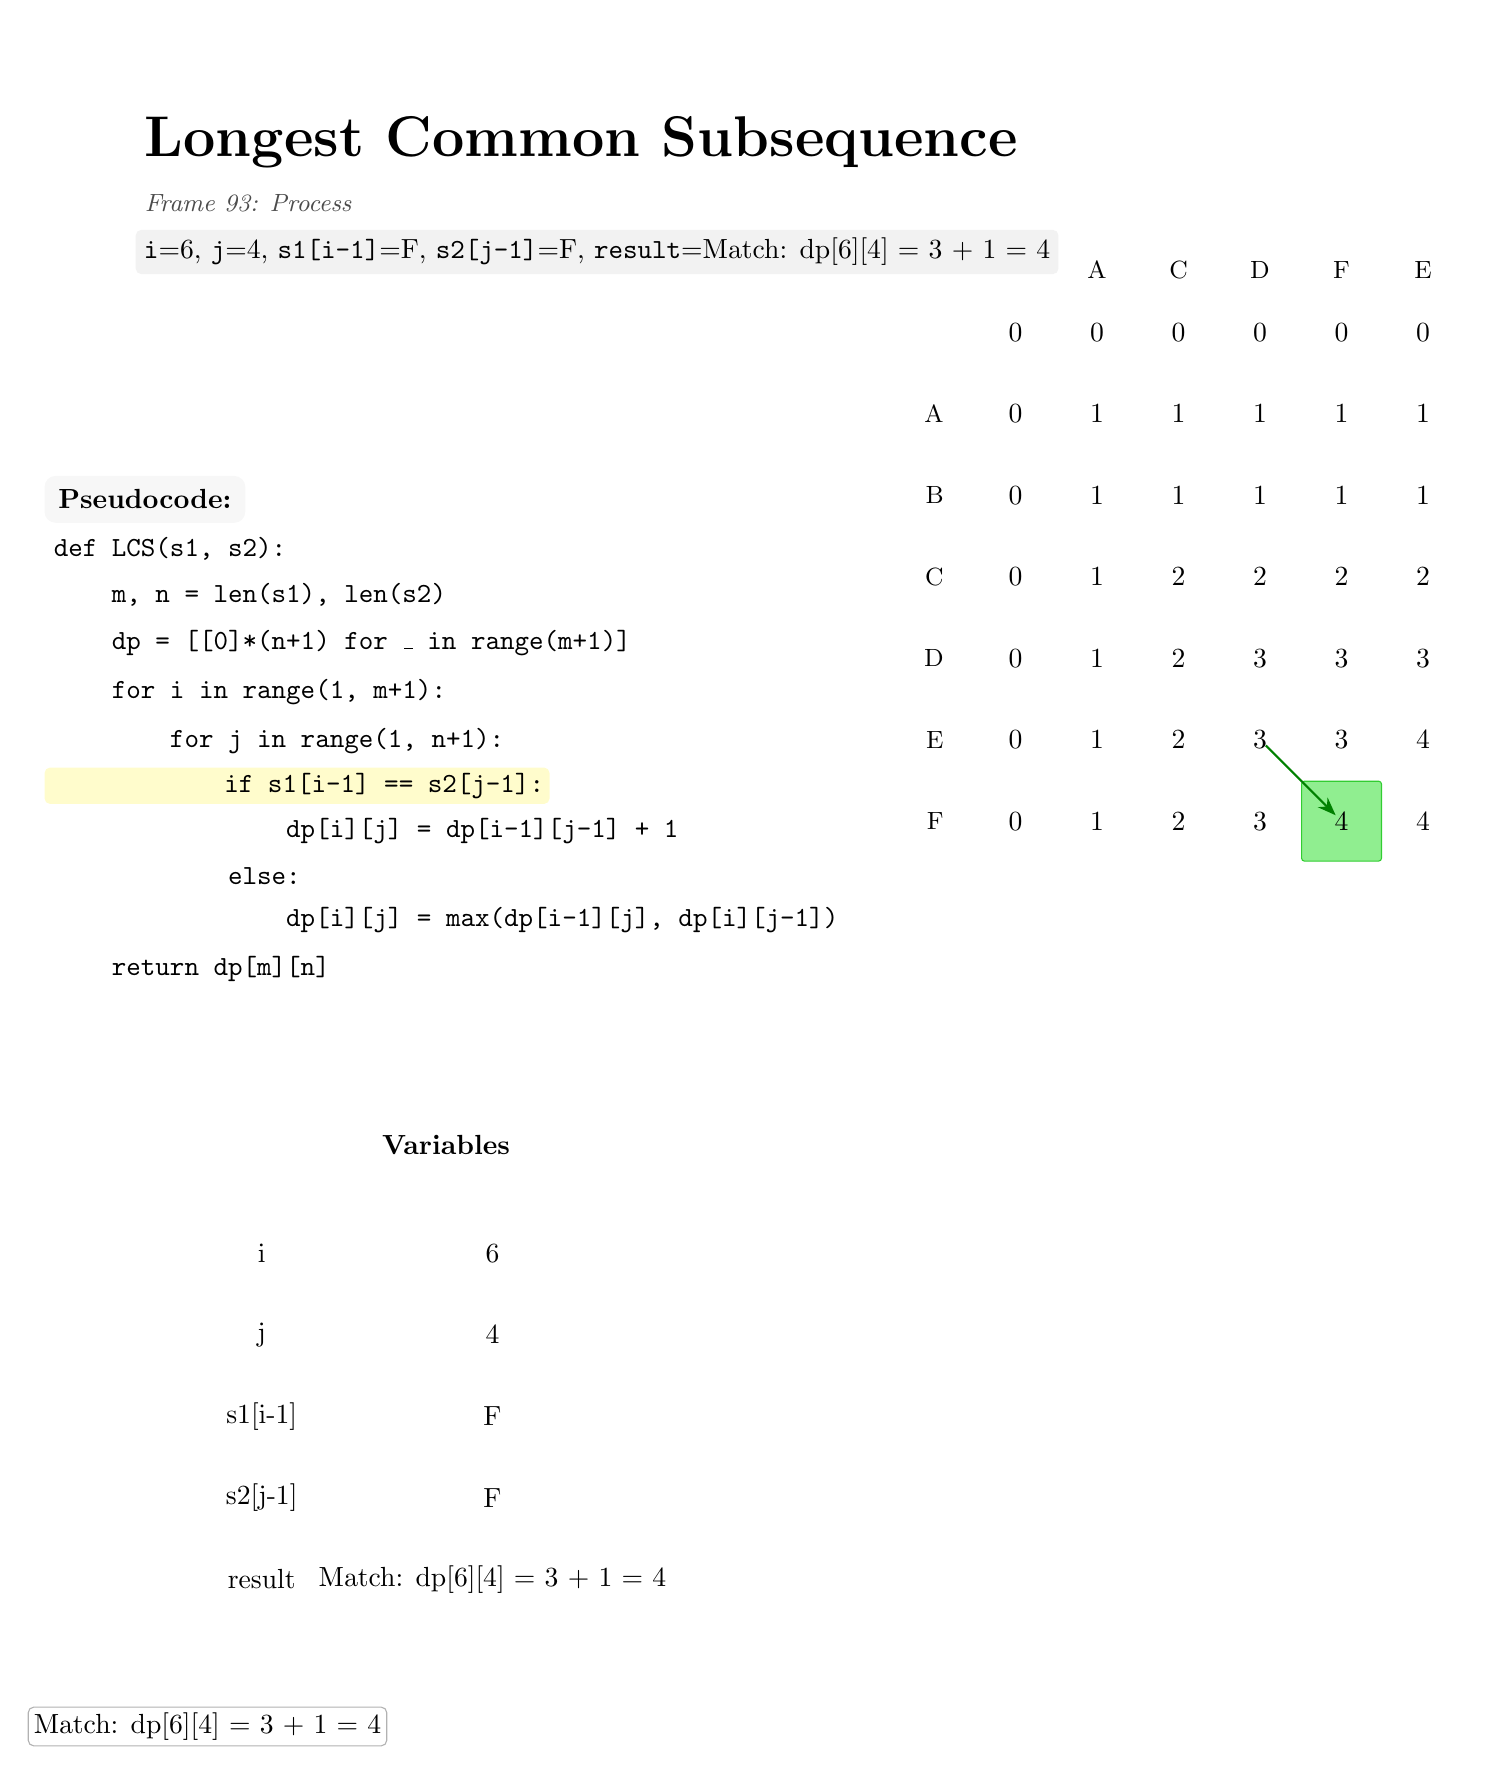
\begin{tikzpicture}[x=1cm, y=1cm, every node/.style={transform shape}]
\path (0, 1.0) -- (0, 0);
\node[font=\huge\bfseries, anchor=north west] (title_node) at (0,0) {Longest Common Subsequence};
\node[font=\small\itshape, color=black!70, below=0.1cm of title_node.south west, anchor=north west] (subtitle_node) {Frame 93: Process};
\node[font=\normalsize, fill=black!5, rounded corners=2pt, inner sep=3pt, below=0.1cm of subtitle_node.south west, anchor=north west] (vars_node) {\texttt{i}=6, \texttt{j}=4, \texttt{s1[i-1]}=F, \texttt{s2[j-1]}=F, \texttt{result}=Match: dp[6][4] = 3 + 1 = 4};
\node (left_col_start) [below=0.8cm of vars_node.south west, anchor=north west] {};
\node[font=\bfseries, anchor=west, fill=black!3, rounded corners, inner sep=5pt] (pseudo_title) [below=1.5cm of left_col_start, anchor=north] {Pseudocode:};
\node[code_line, font=\ttfamily, anchor=north west] (pseudo_line_0) at ($(pseudo_title.south west) + (0, -0.05)$) {\hspace*{0.0em}def LCS(s1, s2):};
\node[code_line, font=\ttfamily, anchor=north west] (pseudo_line_1) at ($(pseudo_line_0.south west) + (0, -0.05)$) {\hspace*{2.0em}m, n = len(s1), len(s2)};
\node[code_line, font=\ttfamily, anchor=north west] (pseudo_line_2) at ($(pseudo_line_1.south west) + (0, -0.05)$) {\hspace*{2.0em}dp = [[0]*(n+1) for \_ in range(m+1)]};
\node[code_line, font=\ttfamily, anchor=north west] (pseudo_line_3) at ($(pseudo_line_2.south west) + (0, -0.05)$) {\hspace*{2.0em}for i in range(1, m+1):};
\node[code_line, font=\ttfamily, anchor=north west] (pseudo_line_4) at ($(pseudo_line_3.south west) + (0, -0.05)$) {\hspace*{4.0em}for j in range(1, n+1):};
\node[code_highlight, font=\ttfamily, anchor=north west] (pseudo_line_5) at ($(pseudo_line_4.south west) + (0, -0.05)$) {\hspace*{6.0em}if s1[i-1] == s2[j-1]:};
\node[code_line, font=\ttfamily, anchor=north west] (pseudo_line_6) at ($(pseudo_line_5.south west) + (0, -0.05)$) {\hspace*{8.0em}dp[i][j] = dp[i-1][j-1] + 1};
\node[code_line, font=\ttfamily, anchor=north west] (pseudo_line_7) at ($(pseudo_line_6.south west) + (0, -0.05)$) {\hspace*{6.0em}else:};
\node[code_line, font=\ttfamily, anchor=north west] (pseudo_line_8) at ($(pseudo_line_7.south west) + (0, -0.05)$) {\hspace*{8.0em}dp[i][j] = max(dp[i-1][j], dp[i][j-1])};
\node[code_line, font=\ttfamily, anchor=north west] (pseudo_line_9) at ($(pseudo_line_8.south west) + (0, -0.05)$) {\hspace*{2.0em}return dp[m][n]};
\node[fit=(pseudo_title) (pseudo_line_0) (pseudo_line_1) (pseudo_line_2) (pseudo_line_3) (pseudo_line_4) (pseudo_line_5) (pseudo_line_6) (pseudo_line_7) (pseudo_line_8) (pseudo_line_9), inner sep=0.2cm] (pseudo_block) {};
\node[font=\bfseries, below=1.5cm of pseudo_block] (title_vars_panel) {Variables};
\matrix (matrix_vars_panel) [below=0.5cm of title_vars_panel, matrix of nodes, nodes={minimum size=1.0cm, anchor=center}, column sep=1pt, row sep=1pt] {
i & 6 \\
j & 4 \\
s1[i-1] & F \\
s2[j-1] & F \\
result & Match: dp[6][4] = 3 + 1 = 4 \\
};
\node[fit=(title_vars_panel) (matrix_vars_panel-1-1), inner sep=0.1cm] (aux_view_block_0) {};
\node[fit=(title_vars_panel) (matrix_vars_panel-1-1), inner sep=0.1cm] (first_aux_view_block) {};
\node[fit=(title_vars_panel) (matrix_vars_panel-1-1), inner sep=0.1cm] (last_aux_view_block) {};
\node[fit={(first_aux_view_block) (last_aux_view_block)}, inner sep=0.1cm] (aux_full_block) {};
\node[fit={(pseudo_block) (aux_full_block)}, inner sep=0pt] (left_column_box) {};
\node (right_col_start) at ($(left_column_box.north east) + (4.5cm, 0)$) {};
\begin{scope}[shift={($(right_col_start) + (0, 0.0)$)}]
\matrix (dp_table) at (0, -1.5) [matrix of nodes, nodes={minimum size=1.0cm, anchor=center}, column sep=1pt, row sep=1pt] {
0 & 0 & 0 & 0 & 0 & 0 \\
0 & 1 & 1 & 1 & 1 & 1 \\
0 & 1 & 1 & 1 & 1 & 1 \\
0 & 1 & 2 & 2 & 2 & 2 \\
0 & 1 & 2 & 3 & 3 & 3 \\
0 & 1 & 2 & 3 & 3 & 4 \\
0 & 1 & 2 & 3 & 4 & 4 \\
};
\node[font=\small] at (dp_table-1-1.north) [yshift=8pt] { };
\node[font=\small] at (dp_table-1-2.north) [yshift=8pt] {A};
\node[font=\small] at (dp_table-1-3.north) [yshift=8pt] {C};
\node[font=\small] at (dp_table-1-4.north) [yshift=8pt] {D};
\node[font=\small] at (dp_table-1-5.north) [yshift=8pt] {F};
\node[font=\small] at (dp_table-1-6.north) [yshift=8pt] {E};
\node[font=\small, anchor=east, xshift=-8pt] at (dp_table-1-1.west) { };
\node[font=\small, anchor=east, xshift=-8pt] at (dp_table-2-1.west) {A};
\node[font=\small, anchor=east, xshift=-8pt] at (dp_table-3-1.west) {B};
\node[font=\small, anchor=east, xshift=-8pt] at (dp_table-4-1.west) {C};
\node[font=\small, anchor=east, xshift=-8pt] at (dp_table-5-1.west) {D};
\node[font=\small, anchor=east, xshift=-8pt] at (dp_table-6-1.west) {E};
\node[font=\small, anchor=east, xshift=-8pt] at (dp_table-7-1.west) {F};
\begin{pgfonlayer}{background} \node[cell_match_cell, fit=(dp_table-7-5), inner sep=0pt] {}; \end{pgfonlayer}
\draw[dep_match_arrow, thick, ->, shorten >=3pt, shorten <=3pt] (dp_table-6-4.center) to (dp_table-7-5.center);
\end{scope}
\path (current bounding box.south) -- ++(0,-1.0) coordinate (comments_start);
\node[comment_default_comment, align=left, anchor=north west] (comment_node_0) at (current bounding box.west |- comments_start) {Match: dp[6][4] = 3 + 1 = 4};
\path (title_node.north west) -- (current bounding box.south east);
\end{tikzpicture}
\end{document}
